\section{Влияние скорости охлаждения образца на результирующий профиль}

Важной особенность метода СЭЛТР является тот факт, что формирование профиля завершается только при охлаждении образца до температуры около 80~$^\circ$C, что занимает некоторое время после окончания экспонирования. В данном разделе приводятся результаты моделирования конечного профиля линии, получаемой методом СЭЛТР, при значений скорости охлаждения образца, отличающихся от скорости его охлаждения в эксперименте.

Как и ранее, считалось, что экспонирование резиста в процессе СЭЛТР производится ``в кадр'' с параметрами кадра, описанными в разделе~\ref{sec:verification}. В качестве исходных параметров экспонирования были приняты $T$ = 130~$^\circ$C, $t_\mathrm{exp}$~=~100~c, $I$ = 4.56 нА, начальная толщина слоя ПММА считалась равной 500 нм, а зависимость температуры образца от времени при охлаждении изначально описывалась экспериментальной кривой охлаждения, приведенной на рисунке~\ref{fig:exp_cooling} (профиль линии, получаемой в этих условиях, приведен на рисунке~\ref{fig:DEBER_4_profiles} в)). При данных параметрах процесса СЭЛТР в резисте на момент остывания остаются микрополости, что обеспечивает меньший радиус кривизны профиля в центре линии по отношению к случаю полного заполнения микрополостей (рисунки~\ref{fig:DEBER_4_profiles} а), б) и г)).

На рисунке~\ref{fig:DEBER_cooling} приведены промоделированные профили линий, полученных методом СЭЛТР при одинаковых условиях экспонирования, описанных выше, но с разными скоростями охлаждения образца после экспонирования. Результаты моделирования демонстрируют заметное влияние микрополостей в слое резиста на форму профиля, особенно в центре линии. Исходя из того, что среднеквадратичное отклонение точек промоделированных профилей в центре линии при наличии микрополостей составляет около 15 нм, требование к стабильности скорости охлаждения образца может быть сведено к максимально допустимой флуктуации скорости охлаждения образца, равной 0.1~$^\circ$C/с (аналогично максимально допустимым значения флуктуаций параметров экспонирования, полученным ранее).

\begin{figure}[h]
	\begin{minipage}{0.48\textwidth}
		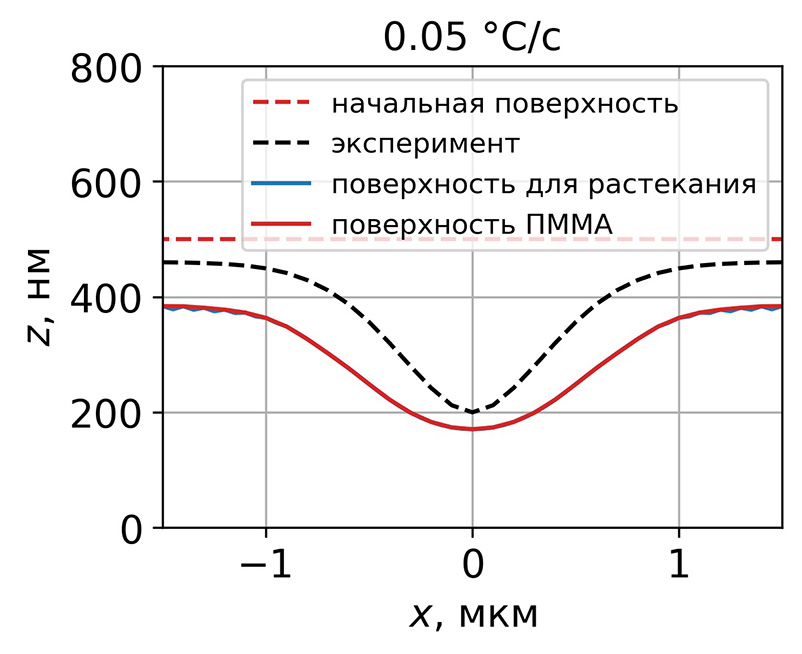
\includegraphics[width=\linewidth]{DEBER_cooling/cooling_0p05_200} \\
		\vspace{-13em} \\ \text{\hspace{0em} a}) \\ \vspace{13em}
	\end{minipage}
	\begin{minipage}{0.48\textwidth}
		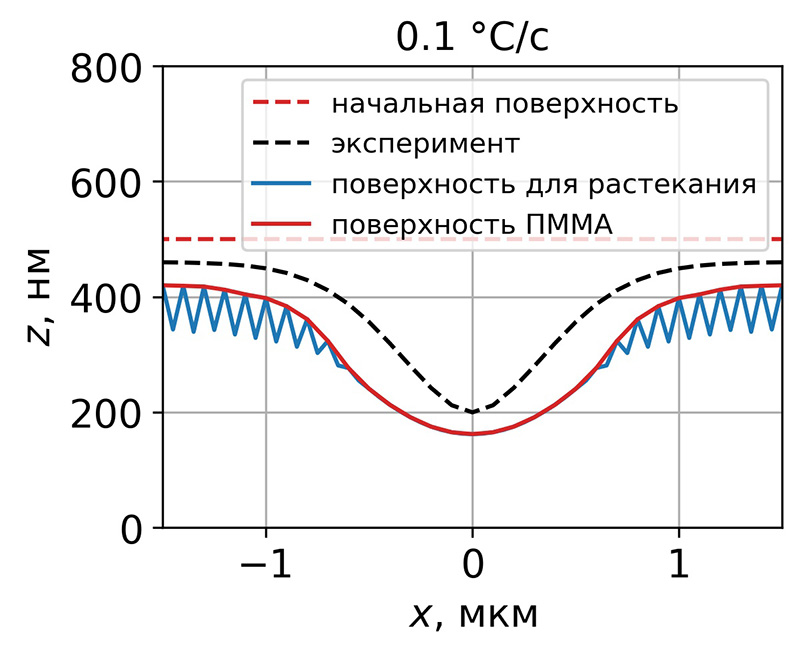
\includegraphics[width=\linewidth]{DEBER_cooling/cooling_0p1_200} \\
		\vspace{-13em} \\ \text{\hspace{-0.1em} б}) \\ \vspace{13em}
	\end{minipage}
	
	\vspace{-3em}
	
	\begin{minipage}{0.48\textwidth}
		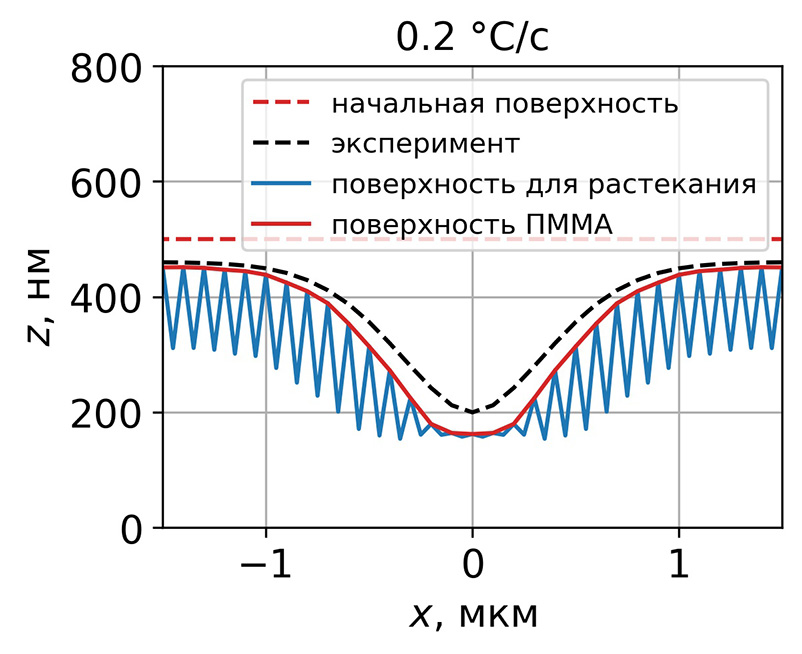
\includegraphics[width=\linewidth]{DEBER_cooling/cooling_0p2_200} \\
		\vspace{-13em} \\ \text{\hspace{0em} в}) \\ \vspace{13em}
	\end{minipage}
	\begin{minipage}{0.48\textwidth}
		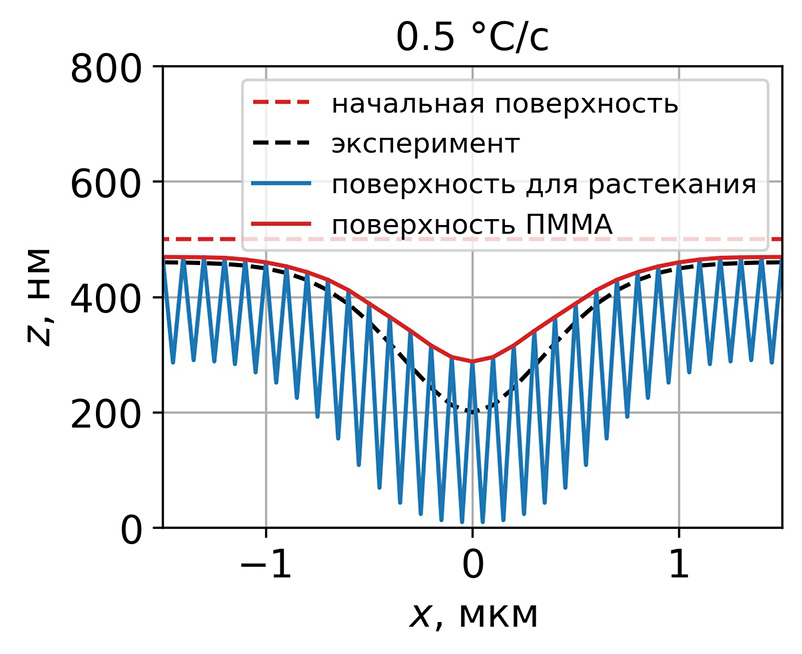
\includegraphics[width=\linewidth]{DEBER_cooling/cooling_0p5_200} \\
		\vspace{-13em} \\ \text{\hspace{-0.1em} г}) \\ \vspace{13em}
	\end{minipage}
	\vspace{-3em}
	\caption{Промоделированные профили, получаемые методом СЭЛТР при $T$ = 130~$^\circ$C, $t_\mathrm{exp}$ = 100 c и $I$ = 4.56 нА. Скорость охлаждения образцов варьируется в пределах 0.05--0.5 $^\circ$C.}
	\label{fig:DEBER_cooling}
%	\vspace{0.5em}
\end{figure}
